\documentclass{sig-alternate-05-2015}
\usepackage{float}
\setcounter{topnumber}{10}
\def\topfraction{.9}
\setcounter{bottomnumber}{10}
\def\bottomfraction{.9}
\setcounter{totalnumber}{10}
\def\textfraction{0}
\def\floatpagefraction{.9}
\setcounter{dbltopnumber}{10}
\def\dbltopfraction{.9}
\def\dblfloatpagefraction{.9}

\begin{document}

\title{CS265 Final Project: LSM-tree gradient descent}
\subtitle{Optimizing Memory Allocation Between Memtable, Cache, and Bloom Filters}
\numberofauthors{3}
\author{
\alignauthor
Mali Akmanalp\\
       \affaddr{Harvard University}\\
       \email{mea590@g.harvard.edu}
\alignauthor
A. Sophie Hilgard\\
       \affaddr{Harvard University}\\
       \email{ash798@g.harvard.edu}
\alignauthor Andrew Ross\\
       \affaddr{Harvard University}\\
       \email{andrew\_ross@g.harvard.edu}}

\date{\today}

\maketitle

\section{Introduction}

Tuning data systems is hard. Even for systems like key-value stores that only
support the most minimal API (\texttt{put} and \texttt{get}), the possibilities
are often overwhelming. The developers of RocksDB \cite{facebook:rocksdb}, a
popular and powerful LSM tree-based key-value store, freely admit that
``configuring RocksDB optimally is not trivial,'' and that ``even [they] as
RocksDB developers don't fully understand the effect of each configuration
change'' \cite{rocksdb-tuning-guide}. Additionally, the optimality of a
database configuration depends on that database's \textit{workload}, which is
rarely known in advance.  There has been recent work \cite{monkey} in
determining the optimal memory allocation for bloom filters in LSM trees in
terms of worst-case analysis and with respect to a number of basic workloads,
but realistic key-value store workloads, which have been analyzed e.g. for
Facebook \cite{characterizing-memcached}, exhibit enormous complexities with
respect to time, skewness, and key repeatability which have not been factored
in.

Our goal is somewhat ambitious -- building on Monkey \cite{monkey}, we seek to
optimize not just bloom filter memory allocation but memory allocation across
the entire LSM tree; that is, given a total amount of memory $M$, we want to
choose an amount of cache memory $M_{cache}$, buffer/memtable memory
$M_{table}$, and bloom filter memory $M_{bloom}$ such that
$M=M_{cache}+M_{table}+M_{bloom}$ and disk accesses across the LSM tree are
minimized. Furthmore, we want to perform this optimization with respect to a
diverse set of workloads that we model as stochastic processes.

\section{Stochastic Workloads}

To benchmark our results, rather than generating workloads which are fixed sets
of queries, we define a diverse set of random workload generating classes.
Each class is highly configurable and often hierarchical in their probabilistic
models.  From them, we randomly regenerate workloads with similar high-level
characteristics but different queries. This strategy does not necessarily
guarantee realism but helps us avoid "overfitting" to a particular set of
queries. The workloads we define contain many simple distributions that are
standard in the literature, along with more complex, time-varying workloads
(inspired by \cite{characterizing-memcached} and \cite{linkbench}) that attempt
to mimic more realistic settings.

\subsection{Simple workloads}

\textbf{Uniform} queries will be drawn uniformly from keys $k \in
\{0,1,...,K\}$, where $K$ is a maximum key (that we explore varying).
The case of uniformly distributed queries is often one in
which the cache is unhelpful (unless $M_{cache} > K$), but in practice may be
unrealistic. Nevertheless, this is the scenario that many analyses assume for
calculations of big-O complexity.

\textbf{Round-Robin} queries are drawn deterministically using $k_i = (i \mod
K)$, i.e. we iteratively draw each key in sequence, then repeat.
This is also a bad case for our key-value store in its default configuration;
the fact that a key has been recently written or read is actually a
contraindication we will access it again.

\textbf{80-20} queries (which are considered in \cite{monkey}) are drawn such
that 20\% of the most recently inserted keys constitute 80\% of the lookups.
This is a simple model we will be able to analyze analytically that exhibits
more realistic skew.

\textbf{Zipf} queries are distributed according to a Zipf or zeta distribution,
where the probability of a given key $k$ is $\propto \frac{1}{k^s}$, where $s
\in (1, \infty)$ describes the skewness of the distribution; in the limit
$s=1$, it is uniform with $K=\infty$. Zipf-distributed queries are considered
in \cite{art} as another simple proxy for realistically skewed queries.

For all the above queries, when we draw a particular key for the first time, we
will insert it into the database as a write, and subsequently we will either
look it up or update it with probability $w$.

Examples of these workloads can be seen in the first row of Figure
\ref{fig:workloads}.

\begin{figure*}[!htb]
\begin{center}
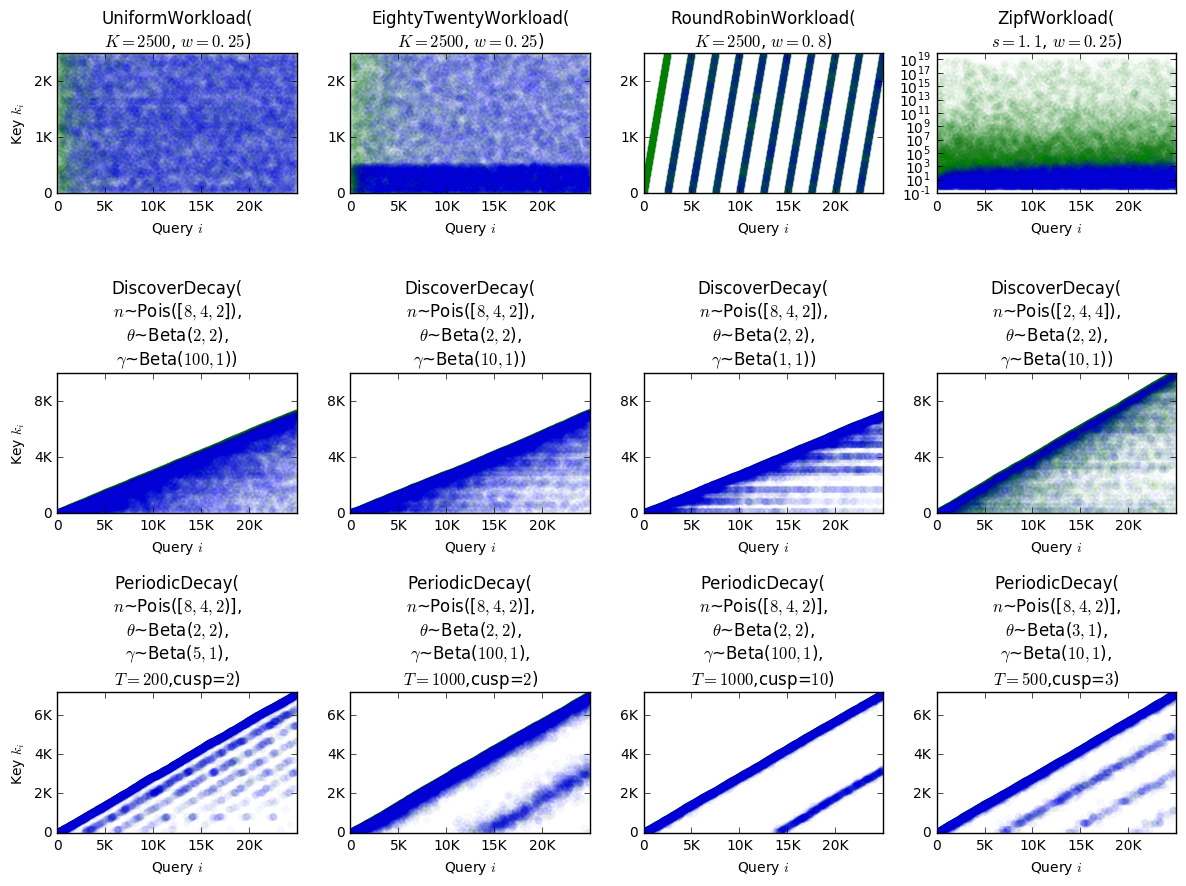
\includegraphics[width=0.81\textwidth]{workloads.png}
\end{center}
\caption{Example workloads we generated for benchmarking. The first row
  contains simple workloads where the distribution of key popularities does not
  change over time, and where the read/write ratio is a uniform probability.
  The second row contains Discover-Decay workloads, which add/read/update keys
  according to Poisson processes and simulate popularity decays over time. The
  third row is a modified version of Discover-Decay that adds a periodic signal
  to the decaying popularity with a configurable period and cusp sharpness. Blue
  dots represent reads and green dots represent writes or updates.}
\label{fig:workloads}
\end{figure*}

\subsection{Complex workloads}

\textbf{Discover-Decay} queries are distributed according to the following
stochastic process, inspired by the Chinese Restaurant process \cite{crp} but
with time decay: with every passing time step, we draw a number of reads $n_r$,
writes $n_w$, and updates $n_u$ assuming queries arrive according to Poisson
processes with configurable rates: \[
\begin{split}
  n_r & \sim \textrm{Pois}(\lambda_r) \\
  n_w & \sim \textrm{Pois}(\lambda_w) \\
  n_u & \sim \textrm{Pois}(\lambda_u)
\end{split}
\]

Poisson processes are a reasonable choice for modeling the arrivals of database
queries or in general the number of events that occur in a continuous time
interval, and have been shown to be appropriate for database queries
\cite{poisson-db1,poisson-db2,poisson-db3}; they are the model that emerges
if we make no special assumptions (i.e. maximum entropy) about the
length of time between queries.  A more realistic model might increase and
lower the rate to mimic the diurnal and weekly cycles seen in
\cite{characterizing-memcached}, but especially on short timescales, Poisson
processes should be much more realistic than assuming a uniform arrival rate
(which we did above).

Once we've drawn our $n_w$ new keys $k_i$, we assign them an initial popularity
$$
\theta_{i} \sim \textrm{Beta}(a_\theta,b_\theta)
$$
\noindent with a random decay rate
$$
\gamma_i \sim \textrm{Beta}(a_\gamma,b_\gamma),
$$
which is the factor by which they exponentially decay each subsequent time
step. At any time $t$, the popularity of each key is given by $p(k_i,t) \propto
\theta_i\gamma_i^{t-t_i}$, where $t_i$ is when the key was inserted. We use
these time-dependent popularities to draw each of our $n_r$ reads and $n_u$
updates from $\textrm{Mult}(\{p(k_i,t)\})$. Examples can be seen in Figure
\ref{fig:workloads}.

\begin{figure}[!htb]
\begin{center}
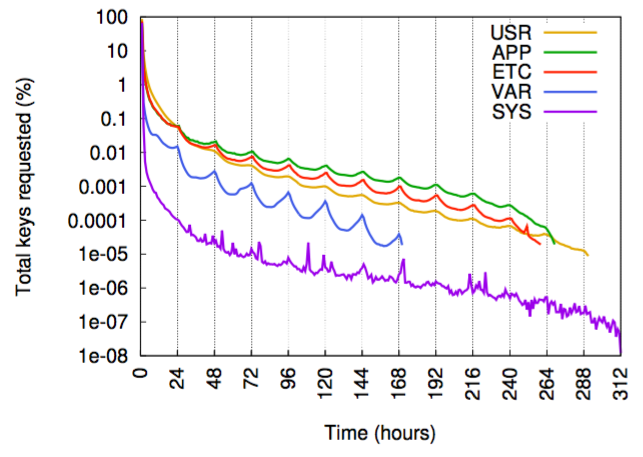
\includegraphics[width=0.4\textwidth]{cuspity.png}
\end{center}
\caption{Key reuse histogram from \cite{characterizing-memcached} showing the
  popularity of keys requested multiple times as a function of the number of
  hours since the previous access for a number of real key-value store
  workloads from Facebook. Note the overall trend of exponential decay with a
  sharply periodic subsignal on a 24-hour scale (for most workloads).}
\label{fig:memcached-decay}
\end{figure}

\textbf{Periodic Decay} workloads are a simple modification of the
Discover-Decay model where $p(k_i,t)$ now depends not only on the decay rate
$\gamma_i$ but also on a periodic function of the key's age $t-t_i$.  To mimic
the combination of exponential decay and sharp periodic peaking we see in
\cite{characterizing-memcached} (from which we reproduce the relevant plot in
Figure \ref{fig:memcached-decay}), we multiply $\theta_i\gamma_i^{t-t_i}$ by an
inverse cycloid function with period $T$, clamped from 0 to 1, and taken to a
configurable power (to make the cusps sharper or duller) that we call the
cycloid's \texttt{cuspity}. Examples can be seen in row 3 of Figure
\ref{fig:workloads}.

\pagebreak

\section{The workload matters}

The first important takeaway is that how much memory we should allocate to the cache,
buffer, and bloom filters is highly dependent on the workload.

To investigate this, we wrote Python code to simulate how an LSM tree with a
variably sized cache, memtable, disk layers, and bloom filters performs for an
arbitrary sequence of queries \cite{lsmulator}. In particular, we count disk
accesses (the main performance bottleneck for an LSM tree) as well as
statistics about the utility of each component. For the experiments below, we
started from an empty LSM tree, but future experiments should pick a sensible
intermediate state.

Figure \ref{fig:period-lsmulations} shows how the number of disk accesses (on a log
color scale) changes as we run a full simulation along different allocations of
8000 bytes (corresponding to the amount of memory needed to store 1000 64-bit
entries, and assuming a page size of 2048 bytes), with about 50000 queries
for each simulation. We allocate these 8000 bytes using a 400-byte grid spacing
along the simplex of possible splits, and test using both baseline (equal bits-per-entry) and Monkey
bloom filter allocations \cite{monkey}.

\begin{figure}[!htb]
\begin{center}
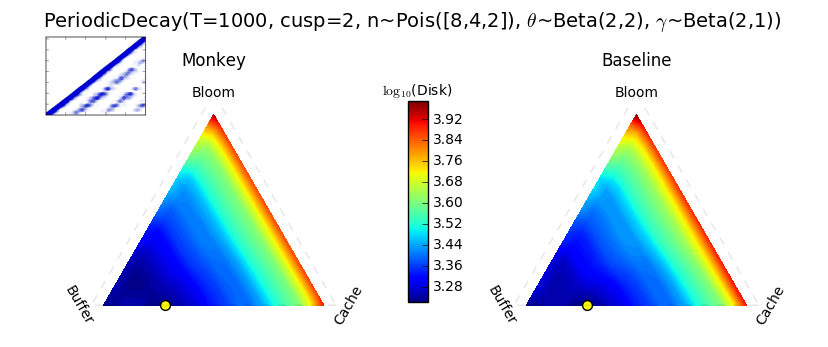
\includegraphics[width=0.5\textwidth]{period2.png}
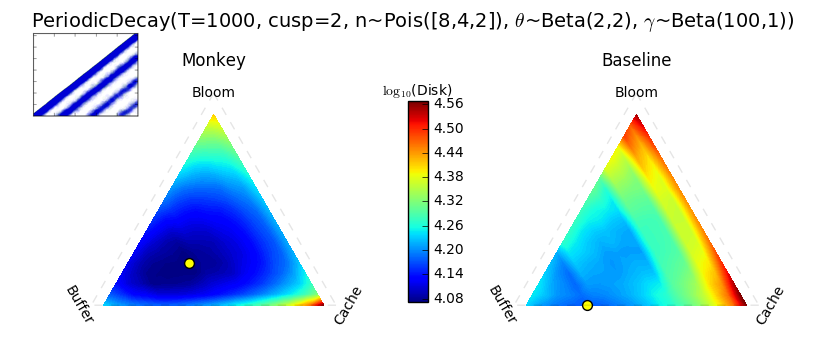
\includegraphics[width=0.5\textwidth]{period1.png}
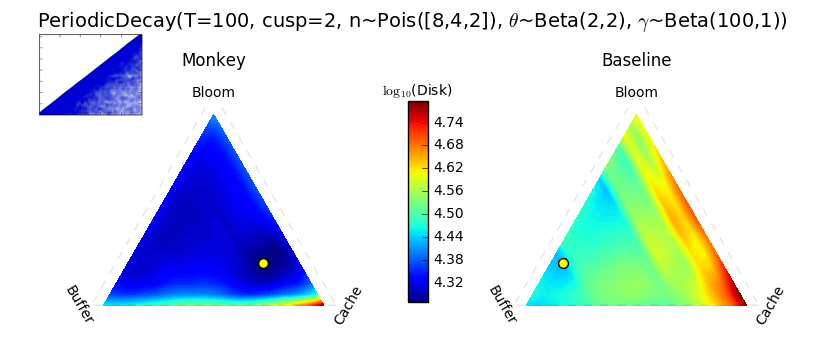
\includegraphics[width=0.5\textwidth]{period3.png}
\end{center}
\caption{Sets of simulation results for three variants of the Periodic Decay
workload (shown in the top-left corner of each set of plots). The minimum,
plotted as a yellow dot, is determined by exhaustive search over the simplex
of possible allocations. Note how the best allocation is highly dependent
on the workload, and how Monkey always outperforms the baseline allocation.}
\label{fig:period-lsmulations}
\end{figure}

We will include results for many more workloads than just the Periodic Decay
variants shown in Figure \ref{fig:period-lsmulations}, but even just those
three are sufficient to illustrate a variety of takeaways. For the top plot,
whose workload consists primarily of reads of very recently added keys but with a few
old popular keys recurring at intervals, we obtain the best results by allocating
most of our memory to the buffer (for reading recently added keys), but saving a little
bit for the cache (for the old but popular recurring keys). The bloom filters are
actually useless to us, and as such, it does not matter whether we use Monkey or not
to allocate our bloom filters.

The middle plot shows a case where old keys recur in greater numbers (because
the decay rates are lower), so the cache alone does not suffice, although it
still helps for the most popular old keys (since there is still a spread). Now
we transition into a regime where the bloom filter also helps, but only when we
use Monkey to allocate memory optimally across the filters. The baseline
allocation is not quite good enough to move the optimum away from the pure
cache and buffer configuration (and the optimization landscape is starting to
look non-convex).

The bottom plot, which has a much higher periodic frequency along with slow
decay, shows non-convexity or multimodality in the Monkey results; one local
minimum involves allocating a significant amount of memory to the cache and
less to the buffer, while another local minimum allocates memory to the buffer
(plus slightly more bloom) and much less to the cache. The multimodality makes
sense, because our LSM tree affords us multiple strategies for avoiding disk
accesses on popular keys; one is to focus on recent keys, which are more likely
to be popular, and another is to focus on keys which remain popular for a long
time. Interestingly, in the baseline case, the cache strategy no longer works
well, perhaps because it implicitly relied on the bloom filters in some way.
Note also the discontinuities that occur along the buffer direction, which are
a result of the number of layers sharply changing with the buffer size.

These results demonstrate (1) there are many qualitatively distinct regimes of
optimality in an LSM tree, (2) all components can be important, (3) Monkey
consistently outperforms the baseline bloom filter allocation, even on fairly
exotic workalods, and (4) due to the possibility of non-convexity, globally
optimizing memory allocation might be challenging.

However, the resulting surfaces suggest that at least for some workloads, local
optimization (similar to gradient descent) can be effective for moving toward
an optimal memory allocation without requiring that we iterate through all
possibilities. Additionally, we note that to compute iterative local
optimizations, we do not require that the entire workload be known a priori.
Rather, we can collect minimal statistics throughout the query execution
process and use these to estimate the current value in saved I/Os any marginal
byte of the cache, bloom filters, or memtable is providing. To formulate the
useful statistics, we turn to modeling.

\section{Modeling}

We first consider the case of a uniform query distribution and then show how
the formulation can be generalized to any distribution with an empirical trace.

\subsection{Uniform query distribution}

\noindent Assuming we have
\begin{itemize}
\itemsep-1em
\item $N$ items in total DB \\
\item $E$ size of an entry in bits \\
\item $M$ total memory \\
\item $M_c$ memory allocated to cache \\
\item $M_{buffer}$ memory allocated to buffer\\
\item $P$ size of the buffer in pages \\
\item $B$ entries that fit in a disk page \\
\item $T$ ratio between layers of LSM tree such that \\
\item $L1 = T * B* P$, $L2 =T^2 * B*P $, and so on,
\end{itemize}

\noindent then we can solve for $L$ the total number of layers required to store all the data: \\
$$B*P * \frac{1-T^L}{1-T} = N$$
$$L= \lceil \textrm{log}_{T} \left(\frac{N(T-1)}{PB} + 1\right) \rceil$$


The average cost of a write remains the same as for the basic LSM tree case:

$$
\text{write cost} = \textrm{log}_{T} \frac{N}{BP}
$$

The average cost of a read must be considered probabilistically over all
possible locations of the read item, in this case assuming a uniformly random
distribution of reads:

\begin{itemize}
\item Probability that read is in memtable $= p(\text{MT}) = \frac{B*P}{N}$
\item Probability that read is in cache $= p(\text{cache}) = \frac{M_c/E}{N}$
\item Probability that read is in L1 but not in cache $= p(L1)$ $$= \frac{B*P * T - \frac{B*P*T}{N-B*P} * M_c/E}{N}$$
\end{itemize}

where the numerator is the number of items $B*P*T$ that are in the first layer
minus the proportion of items from that layer that are probabilistically in the
cache already: $$\frac{B*P*T}{N-B*P} * M_c/E$$ and finally where the $N-B*P$
comes from the fact that items already in memtable (L0) are not allowed to
occupy the cache.

Therefore, given a uniform query distribution, the full expected cost in disk
reads of a read is
$$E[C_{\text{uniform}}] = p(\text{MT}) * 0  + p(\text{cache}) * 0 + \sum_{i=1}^L p(L_i) * i$$
$$=\sum_{i=1}^L \frac{B*P * T^i - \frac{B*P*T^i}{N-B*P} * M_c/E}{N} * i$$


\subsection{Bloom Filters}

The previous analysis hasn't yet accounted for the presence of Bloom filters,
which reduce the likelihood we will unnecessarily access a lower layer. For a
Bloom filter of $k$ bits with $h$ independent hash functions $h_1, h_2,...h_h$,
the probability that a given bit is still set to 0 after inserting $n$ keys is 

$$
(1 - \frac{1}{k})^{n*h}
$$
Then the probability of a false positive is 
$$
(1- (1 - \frac{1}{k})^{n*h})^h \approx (1 - e^{-hn/k})^h
$$

We can minimize this over $h$ to find the optimal number of hash functions,
which is $h = \mathrm{ln}(2) * \frac{k}{n}$. Assuming that this is the number
of hash functions $h$ we will use, the probability of a false positive as a
function of the number of bits is then 

$$
(1 - e^{-\mathrm{ln}(2)*k/n*n/k})^{\mathrm{ln}(2) * \frac{k}{n}} = (\frac{1}{2}) ^ {\mathrm{ln}(2) * \frac{k}{n}} \approx (.6185) ^  {\frac{k}{n}}
$$

For an item in any any level $L_i$ of the LSM tree with $i \geq 2$ we can
reduce the expected cost of accessing that item from $i$ by the number of Bloom
filter negatives at any level $j<i$. \\ \\ Then the expected cost of accessing
an item at $L_i$ is  $$\sum_{j=1}^{i-1} p(fp_j) * 1 + 1$$ Where $p(fp_j)$ is
the probability of a false positive for that key at level $j$ and 1 is the cost
of actually accessing the item at level $i$ assuming fence pointers that lead
us to the correct page.

\subsection{Expected Cost with Bloom Filters - Base Case}

Assuming a random distribution of reads, we now consider also the probability that a bloom filter allows us to ignore a level: \\
Expected cost of read for an item in the tree = $$p(mt) * 0  + p(cache) + 0 + \sum_{i=1}^L p(Li) * \sum_{j=1}^{i-1} p(fp_j)$$ \\
Expected cost for a null result read = $\sum_{j=1}^{L} p(fp_j)$

Given a total memory allocation $M$, the total number of bits we can allocate
to bloom filters is $M-M_c = \sum_{i=1}^L m_i$ \\ Then the total formula for
the expected cost of a read in the tree is: 

\begin{multline}
$$E[c] = \sum_{i=1}^{L} \frac{B*P*T^i - \frac{B*P*T^i}{N-B*P} * M_c/E}{N} \\ \cdot \left[ \left(\sum_{j=1}^{i-1} (.6185) ^  {\frac{m_j}{B*P*T^j}}\right) +1 \right]$$ 
\end{multline}

Whereas with a given percentage of null reads in the workload $p_{null}$:

\begin{multline}
$$E[c] = (1-p_{null})\sum_{i=1}^{L} \frac{B*P*T^i - \frac{B*P*T^i}{N-B*P} * M_c/E}{N} \\ \cdot \left[ \left(\sum_{j=1}^{i-1} (.6185) ^  {\frac{m_j}{B*P*T^j}}\right) +1 \right] + p_{null}\sum_{j=1}^{L} p(fp_j)$$
\end{multline}
\begin{multline}
$$E[c] = \sum_{i=1}^{L} (1-p_{null})\frac{B*P*T^i - \frac{B*P*T^i}{N-B*P} * M_c/E}{N} \\ \cdot \left[ \left(\sum_{j=1}^{i-1} (.6185) ^  {\frac{m_j}{B*P*T^j}}\right) +1 \right] + p_{null} \cdot p(fp_i) $$
\end{multline}

\subsection{Expected Cost with Bloom Filters - Generalized Distribution}

Note that in the above, the workload specific factors are the probability that
a read is at any given level and the related probability that any given item
from a level is already in the cache. To compute an empirical estimation of the
probability that any given item is in a layer but not already in the cache, we
can simply keep statistics on the total number of times a key was found in that
layer divided by the total number of (non-null) read queries executed. Then we
can consider the following simplification:

\begin{multline}
$$E[c] = \sum_{i=1}^{L} (1-p_{null})\left[p(L_i) - \frac{p(L_i)}{(N - BP)} * M_c/E \right]\\ \cdot \left[ \left(\sum_{j=1}^{i-1} (.6185) ^  {\frac{m_j}{B*P*T^j}}\right) +1 \right] + p_{null} \cdot p(fp_i) $$
\end{multline}

Taking the derivative with respect to the number of entries in the cache,
$M_c/E$, we get 

$$
- p(L_i)/(N - BP) \cdot \left[ \left(\sum_{j=1}^{i-1} (.6185) ^  {\frac{m_j}{B*P*T^j}}\right) +1 \right]
$$

Which is just the average cost of a read throughout the tree. Then, to keep
statistics on how valuable we expect the cache to be, we maintain statistics on
the average cost of every read performed in the window of interest.

Because the memory allocation problem is discrete anyway, we consider the value
of the bloom filters as a finite difference, that is the approximate value of
any marginal bloom filter bit at layer $k$ will be $E[c | m_k+1] - E[c | m_k]$.
In this computation, all terms in the sums drop out except for those concerning
$m_j$, and we are left with:

\begin{multline}
$$\sum_{i=k}^{L} (1-p_{null})\left[p(L_i) - \frac{p(L_i)}{(N - BP)} * M_c/E \right] \\ \cdot \left\{ \left[ \left( (.6185) ^  {\frac{m_k+1}{B*P*T^j}}\right) +1 \right] - \left[ \left( (.6185) ^  {\frac{m_k}{B*P*T^j}}\right) +1 \right] \right\} \\+ p_{null}  \left( (.6185) ^  {\frac{m_k+1}{B*P*T^j}} - (.6185) ^  {\frac{m_k}{B*P*T^j}}\right)$$
\end{multline}

Rearranging terms, we get:
\begin{multline}
$$\sum_{i=k}^{L} \left[(1-p_{null})\left[p(L_i) - \frac{p(L_i)}{(N - BP)} * M_c/E \right] +  p_{null} \right] \\ \cdot \left( (.6185) ^  {\frac{m_k+1}{B*P*T^j}} - (.6185) ^  {\frac{m_k}{B*P*T^j}}\right)$$
\end{multline}

Where this is exactly the number of times the given bloom filter is accessed
times the difference in the theoretical false positive rates given memory
allocations $m_j$ and $m_j+1$. Then, to keep statistics on how valuable we
expect any given bloom filter to be, we maintain statistics on the number of
times every bloom filter was accessed in the window of interest.

To estimate the additional value of any marginal memory in the buffer with
respect to reads, we must make a number of simplifications, as $P$, the number
of pages in the buffer, factors into every term in this equation. Further, the
interaction between $P$ and most of the terms is not available in closed form,
in general. Rather, the critical terms $P(L_i)$ we are empirically estimating.
Then, for reasonably large values of $N$ and $P$, we will assume that the bloom
filter false positive rate stays approximately the same, as does the value of
the cache. Then, we consider only the change in I/Os occurring from the altered
probability of any given element occurring in any layer as a result of more
elements being in the memtable. Further, we can provide a simple underestimate
of this by assuming that any items we add to the memtable will be removed from
otherwise occurring in L1, without considering the added value resulting
cascade through all other values in all other layers of the table.

Then, an appropriate estimate of how useful any additional space of memory in
the memtable is is simply the resulting change in $p(L_i)$ * 1 (as any element
at L1 is accessed with a single I/O and no consideration of bloom filter false
positive rates). To estimate how many additional times L1 would be accessed if
we instead allocated the final portion of the memtable to L1, we keep
statistics on how often the final spots of the memtable were accessed in a
read. In practice, these spots are accessed only very infrequently, as the
buffer is accessed only a handful of times at this stage before being flushed.
This statistic might be more helpful on a system with constant compaction
rather than a full layer flush.

For the buffer, we must additionally consider the saved update/insert I/Os.  $$
\text{write cost} = \textrm{log}_{T} \frac{N}{BP} $$ Taking the derivative with
respect to $BP$, the number of items in the buffer, we get $\frac{1}{BP}$ In
discrete terms, this evaluates to $\textrm{log}_{T} \frac{BP}{BP+1}$. 

We consider additionally the fact that I/O savings are lessened by the number
of duplicates inserted, as duplicates will not be merged the full length of the
tree. To take this into account we also keep a statistic for the total number
of duplicates merged over the window of interest and compute the expected
number of saved I/Os for an increase in buffer as $\textrm{log}_{T}
\frac{BP}{BP+1}$ * (number of puts - number of duplicates).  The only
statistics we need to compute this are the empirical number of update queries
and the empirical number of duplicates found and removed over the window of
interest.

\section{Database Stochastic Gradient Descent}

\subsection{Estimating Statistics with $O(1)$ Memory}

\subsection{Testing Accuracy and Variance of Statistics}

To confirm that our estimates are reasonable, we ran 250 simulations for three
separate workloads and compared our estimates of each gradient to the actual
savings for a separate tree with 8 bytes of extra memory in the corresponding
LSM component (against which we ran the same workload). Results can be seen in
Figure \ref{fig:savings}.

\begin{figure*}[!h]
\begin{center}
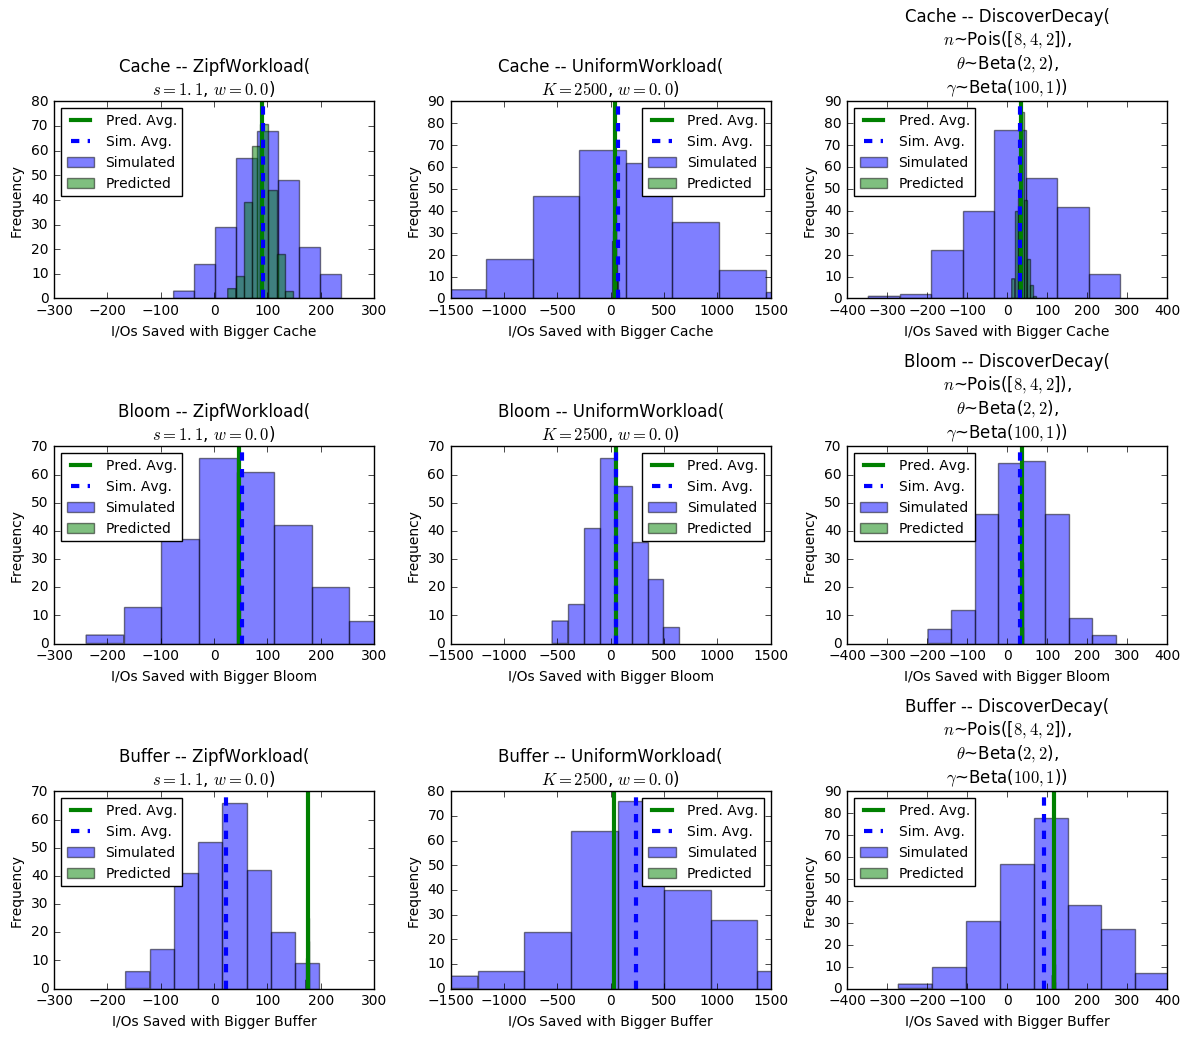
\includegraphics[width=0.8\textwidth]{all-savings.png}
\end{center}
\caption{Light-footprint statistical estimations of the gradient vs. simulated
results for cache, bloom filters, and the buffer on three distinct workloads.}
\label{fig:savings}
\end{figure*}

There is a large amount of variance in the simulated results, both because of
randomness in the separate instantiations of the workload and randomness in
the execution of its queries, but for the most part, our estimates of the average
savings are both precise and accurate.

We do see what appears to be systematic bias in our estimate of the
Discover-Decay memtable savings. This discrepancy may because we do not
properly account for the effects of duplicates in the memtable savings
calculation, which are frequent in this workload, but we do not have a complete
explanation yet. Future work should attempt to resolve this issue, although the
estimate still appears to be reasonably accurate relative to the differences
between component gradients.

\subsection{Results: Database Gradient Descent in Practice}

Now that we have validated the accuracy of our basic gradient estimates, we
evaluate all three of them at every grid point along the simplex of simulated
LSM trees with constant total memory. We then overlay an arrow on top of the
disk access contour plot pointing from the lowest gradient component to the
highest gradient component (signifying that our method suggests moving 8 bytes
from one component to the other). We can then visually inspect these arrows and
see if they generally point us to regions of low disk accesses.

Results for basic workloads can be seen in Figure \ref{fig:basicquiv}.

\begin{figure}[H]
\begin{center}
%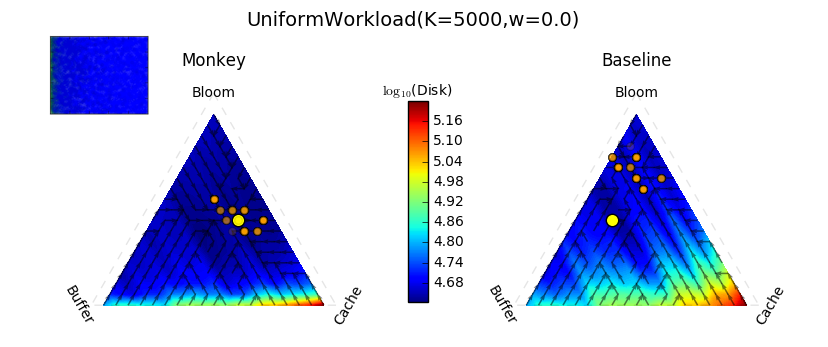
\includegraphics[width=0.5\textwidth]{uniformquiv1.png}
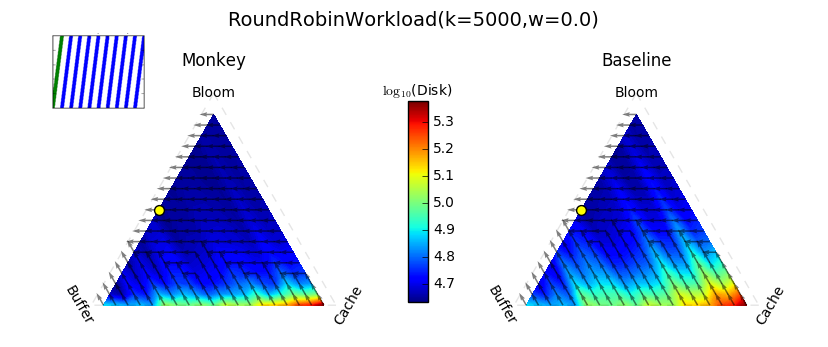
\includegraphics[width=0.5\textwidth]{robinquiv1.png}
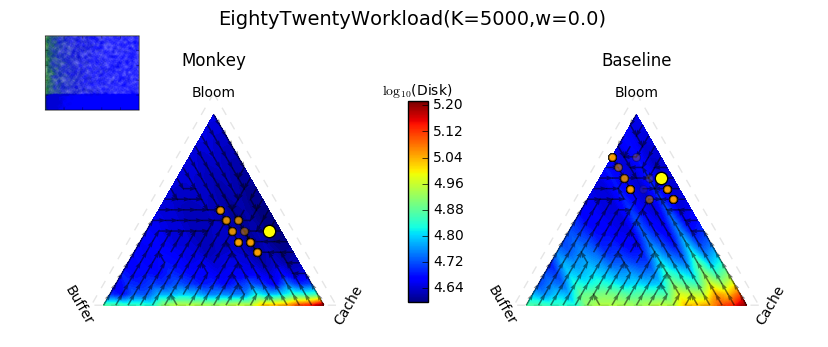
\includegraphics[width=0.5\textwidth]{eightwenquiv1.png}
\end{center}
\caption{Uniform, Round-Robin, and Eighty-Twenty simulation results overlaid with gradient estimates. Following gradients reliably leads to a good configuration, although we tend to undervalue the cache relative to the buffer.}
\label{fig:basicquiv}
\end{figure}

The optimization landscape is again generally non-convex, but Monkey improves both absolute performance and convexity, and following gradient estimates leads us close to the global minimum (perhaps slightly undervaluing the cache). For Zipf workloads in Figure \ref{fig:zipfquiv}, however, we do reach a cache-centric minimum by following gradients.

\begin{figure}[H]
\begin{center}
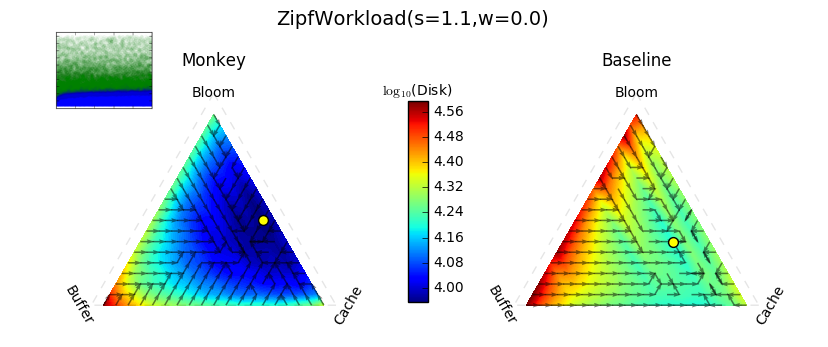
\includegraphics[width=0.5\textwidth]{zipfquiv1.png}
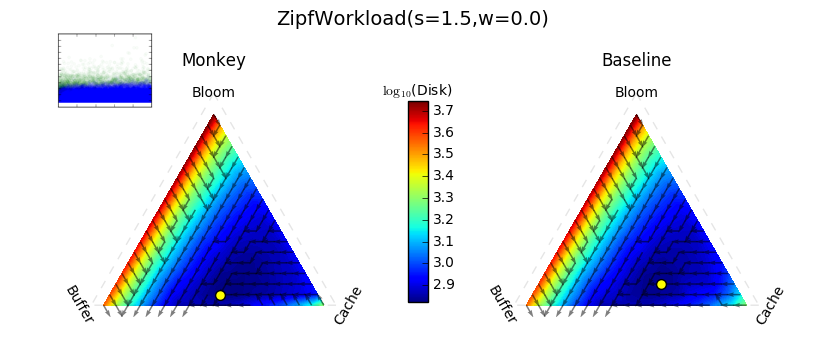
\includegraphics[width=0.5\textwidth]{zipfquiv2.png}
\end{center}
\caption{Zipf simulation results overlaid with gradient estimates for $s=1.1$ (lightly skewed) and $s=1.5$ (highly skewed).}
\label{fig:zipfquiv}
\end{figure}

As we increase the Zipf skewness $s$, we observe a qualitative change in both our simulated results and estimated gradients. At low $s$, the best configuration is a mixture of mostly Bloom filter and cache memory with a relatively small buffer, while at high $s$, Bloom filters are less useful and it is better to allocate more memory to the buffer. This effect may be due to the fact for less skewed workloads, we are more likely to request unpopular keys which may be buried deep in the tree (for which we need Bloom filters), but for highly skewed workloads, we obtain better write and read savings by using the buffer as kind of an auxiliary cache.

For Discover-Decay workloads (Figure \ref{fig:discdecquiv}), we observe a similar transition to the Zipf behavior as we vary skewness, but with a shifted balance between the cache and the buffer (because we have much more frequent inserts and updates). Again, we reliably find a good local or global minimum following gradient estimates.

\begin{figure}[!htb]
\begin{center}
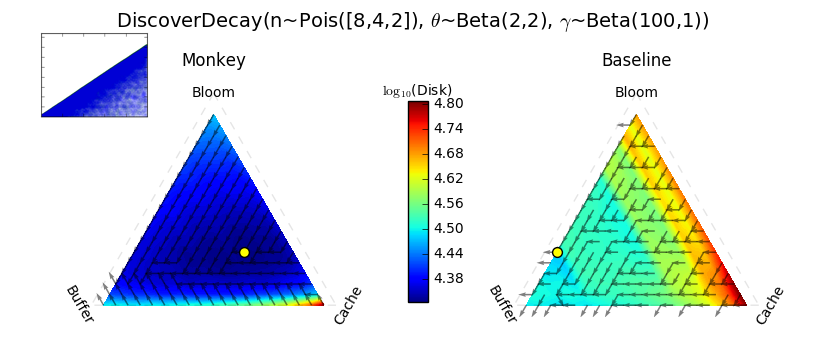
\includegraphics[width=0.5\textwidth]{discdecquiv1.png}
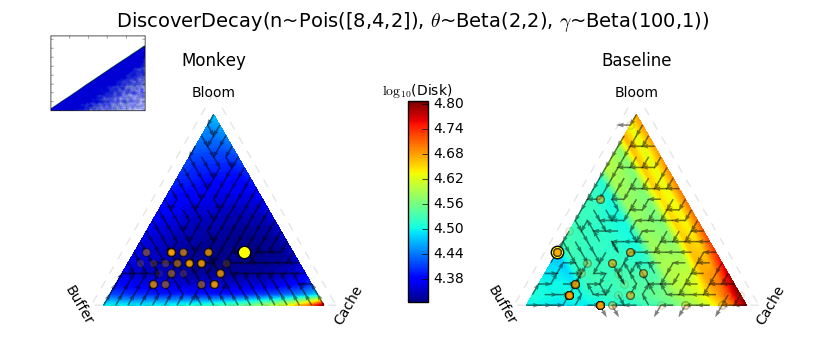
\includegraphics[width=0.5\textwidth]{discdecquiv2.png}
\end{center}
\caption{Discover-Decay simulation results overlaid with gradient estimates for $\gamma\sim\text{Beta}(100,1)$ (lightly skewed) and $\gamma\sim\text{Beta}(2,1)$ (highly skewed).}
\label{fig:discdecquiv}
\end{figure}

Finally, returning to the Periodic Decay workloads, we find that gradients more or less capture the behavior we noted near the beginning of the paper. For lower effective numbers of popular keys (but high temporal locality), we tend to end up allocating most of our memory to the buffer and none to the bloom filters, but as our ``working set'' expands, we are pushed closer to the center of the graph. In the bottom row, the multimodality of the landscape is somewhat visible in the gradient estimates as well.

\begin{figure}[!htb]
\begin{center}
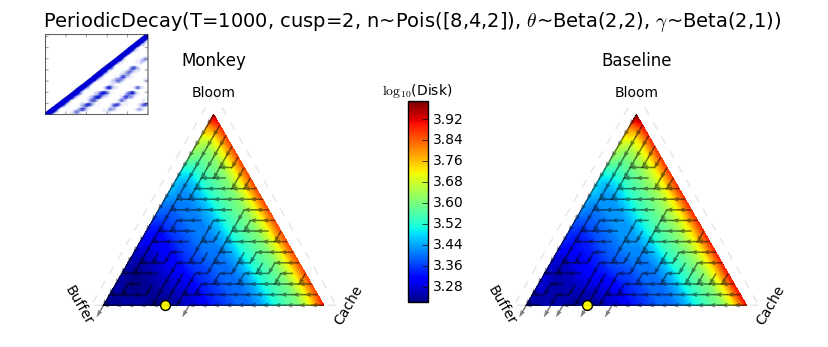
\includegraphics[width=0.5\textwidth]{periodquiv3.png}
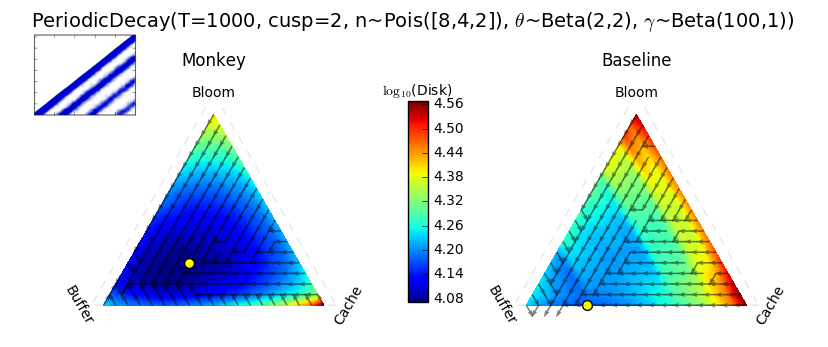
\includegraphics[width=0.5\textwidth]{periodquiv2.png}
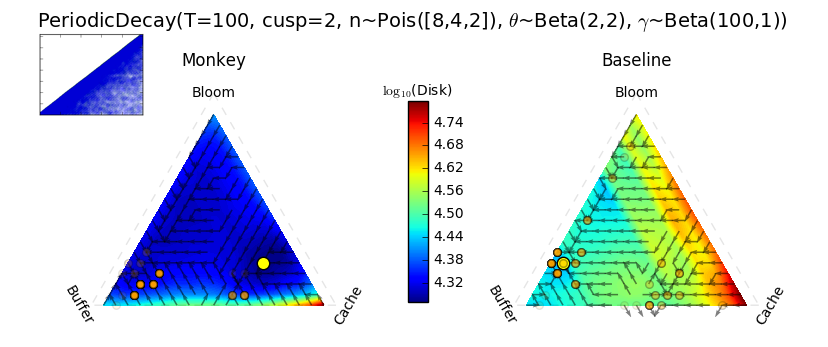
\includegraphics[width=0.5\textwidth]{periodquiv1.png}
\end{center}
\caption{Periodic Decay.}
\label{fig:periodquiv}
\end{figure}

\section{Future Work}

There are many additional optimizations we chose not to address for the moment in this problem. For example, what is the optimal time to reallocate memory? In an environment where we assume full flushing of a given layer and the recomputation of all bloom filters for the layers involved in the flush, it seems like this would be an optimal point to reallocate memory locally among the data structures that are being rewritten anyway. However, this leads to only rare opportunities to recompute deeper layers of the LSM tree, and in practice LSM tree layers are not actually flushed in this `all-at-once' fashion. 

Additionally, the equivalent to a stochastic gradient descent learning rate for our problem is the chunk size of memory that we allow to be reallocated at any calculation point. For now, we consider only the reallocation of the smallest available piece of memory. However, in situations where we have a large amount of conviction in the predictions and they show large potential gains, it might make more sense to reallocate a large block of memory at once. In this case, the reallocation strategy requires more thought than merely taking a chunk from the lowest value data structure and giving it to the highest value data structure. Optimally computing what that reallocation strategy would be would likely require a deeper set of statistics, showing a trend of value over the last portion of any of the data structures, rather than only the last key as we have been using.

Building on the above, there are a number of opportunities for storing histograms rather than simple rolling averages of statistics (in particular, we store a histogram of bloom filter accesses at each stage of bloom filter `fullness' to allow us to calculate the average false positive rate for any number of bits after the fact rather than rolling averages of expected false positive rates for a few potential memory allocations). Histograms are a much heavier statistic than a simple number but provide a greater flexibility in the reallocation stage. More work needs to be done to calculate how much added benefit could be achieved in practice from these costlier statistics and to find scenarios in which they might be worthwhile.

\bibliographystyle{abbrv}
\small
\bibliography{bibliography}

\end{document}
